% !Mode:: "TeX:UTF-8"
%!TEX program  = xelatex

\documentclass[bwprint]{gmcmthesis}
\usepackage[framemethod=TikZ]{mdframed}
\usepackage{subfigure}
\title{基于k-means和PCA的汽车行驶工况构建方法研究}
\baominghao{} %参赛队号
\schoolname{}%学校名称
\membera{} %队员A
\memberb{} %队员B
\memberc{} %队员C
\begin{document}

 %生成标题
 \maketitle

 %填写摘要
\begin{abstract}
本文对题目所给实测数据,经过预处理、建模、分析后得到了所给数据的车辆行驶工况曲线,可以主要归纳整理为以下工作:

\strong{1.对所给数据根据一定的标准进行预处理。}

对于数据缺失,利用python编写函数对三个文件时间序列的缺失长度分布进行观察,由分布变化确定阈值,文件一:13秒,文件二:26秒,文件三:28秒,对于阈值内的缺失数据进行三次样条插值补充,缺失长度大于阈值时,认为进行插值补充的合理性不足,予以去除考虑;利用matlab编写代码,将数据中GPS车速变化梯度过大的位置,根据实际普通轿车的情况(加速大于$-8m/s^2$,小于$3.968m/s^2$),进行插值处理;同时以30秒为长度阈值搜索数据中连续行驶速度低于10km/h的片段,将其与长期停车、低速行驶的情况一同当作怠速处理。上述处理后文件的记录数,文件一:116347,文件二: 108620,文件三:101887。

\strong{2.提取运动学片段数据集。}

采用matlab编程对预处理后的数据进行遍历,将车辆从怠速状态开始至下一个怠速状态开始之间的GPS车速区间当作一个运动学片段,进行片段提取,同时忽略长度小于5秒的运动学片段。得到运动学片段数量,文件一:748,文件二:584,文件三:537。

\strong{3.对运动学片段数据集确定特征变量,特征矩阵降维,并分类。}

考虑到构建行驶工况的目的之一是为了测试汽车的油耗,选取4大类变量,速度变量、加速度变量、驾驶路程与时间和行驶特点变量共23个作为初始特征变量,与所给瞬时油耗进行类内和跨类相关性分析分析筛选,最终保留13个特征变量,见表13,该表即为汽车运动特征评估体系。其次,计算每一个运动片段的特征参数,得到特征运动片段数据集的参数矩阵。对经过均值化处理的特征参数矩阵利用matlab自带的函数库进行主成分分析,得到前5个成分的累计贡献率为85.1\%。最后,基于特征参数前五个主成分的得分矩阵,通过matlab 对运动学片段数据集进行K-均值聚类分析,得到分2、3、4 类的聚类结果,根据结果选择分为2类,第一类运动学片段怠速时间比例较高,平均速度较低,可以反映车辆在城市拥挤道路的行驶情况,第二类运动学片段运行时间比例较高,平均速度较高,可以反映汽车较为顺畅道路行驶情况。

\strong{4.从分类中选取特征片段并组成工况曲线。}

用matlab编写函数,将片段分类在总数据集中的时间占比作为各类典型运动片段的时间权值,设定所需时长1250秒,结合分类运动学片段的平均时间和总时间计算分类所需组成片段数量,分别为5和3;根据各片段与该类总特征向量的相关系数降序排列,取前5\%的运动学片段作为备选集,数量分别为58和34,两个备选集进行遍历组合,选取满足时间长度区间要求,同时与数据集总体的运动学片段特征向量相关系数最大的组合作为所给数据的最优运动学片段组合,进一步得到反映所给数据的汽车行驶工况曲线。

\strong{5.汽车行驶工况评估与验证。}

从特征参数和特征分布两个角度来对比分析构建工况与实际工况。前者用用平均相对误差作为指标进行评价,构建工况与实际工况的个特征参数值见表14,计算得到特征参数的平均相对误差仅为0.0510;后者在定性分析后,用速度-加速度联合分布误差进行定量分析,计算结果为1.55\%。因此,构建工况的代表性得到验证。

完整的研究流程如图一。
\begin{figure}[h] % 插入多张图片并排
\centering
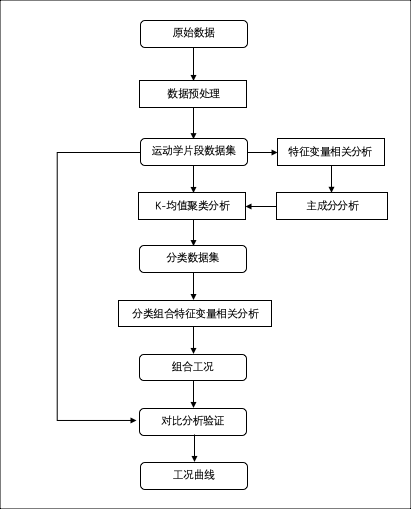
\includegraphics[width=0.60\linewidth,angle=0]{figures/flow.png}
\caption{研究流程}
\label{f1}
\end{figure}


\keywords{工况构建\quad k-means聚类分析\quad 主成分分析\quad  SAFD验证}
\end{abstract}

\pagestyle{plain}

%目录 不推荐加
\tableofcontents
\newpage

\section{问题重述}

\subsection{问题背景}

汽车行驶工况(Driving Cycle)又称车辆测试循环,是描述汽车行驶的速度-时间曲线,体现汽车道路行驶的运动学特征,是汽车行业的一项重要的、共性基础技术,是车辆能耗/排放测试方法和限值标准的基础,也是汽车各项性能指标标定优化时的主要基准。目前,欧、美、日等汽车发达国家,均采用适应于各自的汽车行驶工况标准进行车辆性能标定优化和能耗/排放认证。
然而由于数据不充足、工况构建方法不恰当以及缺乏评价构建工况代表性的方法等,各国目前在用的测试工况与实际车辆的行驶工况都有差距 \cite{c1}。现阶段,我国采用的是法规工况是欧洲的NEDC工况。NEDC工况基于欧洲的交通环境与我国道路上车辆的运行情况有较大差别。如图 2a和图 2b 分别显示的是我国实际工况和NEDC工况,可以看出两者相差很大,由此可知汽车实际油耗和排放与利用法规工况得到的测试值偏差很大\cite{c2}。另一方面,我国地域辽广,各个城市的发展程度、气候条件及交通状况的不同,使得各个城市的汽车行驶工况特征存在明显的不同。因此,基于城市自身的汽车行驶数据进行城市汽车行驶工况的构建研究也越来越迫切,希望所构建的汽车行驶工况与该市汽车的行驶情况尽量吻合,理想情况下是完全代表该市汽车的行驶情况。
\begin{figure}[h] % 插入多张图片并排
\centering
\subfigure[车辆实际工况] { 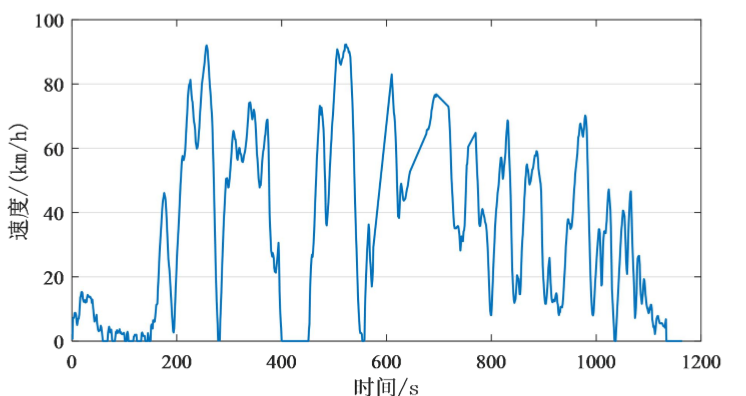
\includegraphics[width=0.42\linewidth,angle=0]{figures/1.png}}
\subfigure[NEDC工况] { 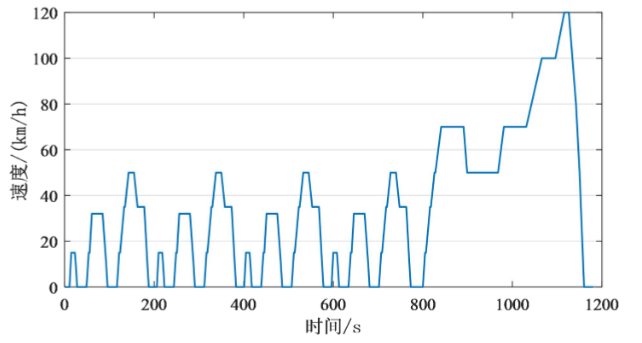
\includegraphics[width=0.42\linewidth,angle=0]{figures/2.png}}
\caption{工况对比}
\label{f1}
\end{figure}

\subsection{问题的提出}
题目提出的问题,即根据所给同一辆车在某城实际道路行驶采集的数据,构建一条能体现参与数据采集汽车行驶特征的汽车行驶工况曲线。总体上需要解决四个方面:;从运动学片段分类中筛选典型运动学片段构建所给数据条件下的合理的汽车行驶工况曲线。解决提出的问题可分为以下几个步骤:
\begin{enumerate}
\item 将所给实测数据进行数据预处理。对于所给数据中的异常数据,如时间不连续,速度梯度的异常值,以及车辆其他异常行驶数据(长期停车、堵车、低速行驶、超长时间怠速)进行预处理。
\item 运动学片段提取。运动学片段是指汽车从怠速状态开始至下一个怠速状态开始之间的车速区间。将预处理后的数据划分为多个运动学片段,组成运动学片段数据集。
\item 汽车行驶工况的构建。将提取得到的运动学片段数据集,采取科学、有效的方法构建一条体现实测数据的车辆行驶工况曲线,时长1200秒至1300秒。
\item 评估分析。构建的汽车行驶工况及汽车运动特征评估体系,将构建的曲线的各运动特征值与预处理后的实测数据进行比较分析,评价构建曲线合理性。
\end{enumerate}

\subsubsection{数据预处理}
对于所给数据中的异常数据,如时间不连续,加速度减速度的异常值,以及车辆异常行驶数据(长期停车、堵车、低速行驶、超长时间怠速)进行预处理,并给出各文件数据经处理后的记录数。

\subsubsection{运动学片段提取}
运动学片段是指汽车从怠速状态开始至下一个怠速状态开始之间的车速区间。请设计合理的方法,将上述经处理后的数据划分为多个运动学片段,并给出各数据文件最终得到的运动学片段数量。

\subsubsection{汽车行驶工况的构建}
从上述处理后得到的运动学片段集合中,依据适当模型和方法,选择运动学片段进行构建题目所给数据工况下的,该城市汽车行驶工况曲线。需要根据数据构建一条时间长度1200至1300秒的能反映参与数据采集的汽车行驶特征的汽车行驶工况曲线,使得该曲线体现的汽车运动特征与代表所采集数据源的相应特征误差尽量小。

\section{问题假设与符号说明}
\subsection{问题假设}
\begin{itemize}
\item 数据插值部分假设车速的变化是在一个运动周期内的连续变化,而不存在急停、急加速这些极端情况
\item 筛除加、减速度异常变化部分假设离群值是噪声,且剔除这些异常值不改变原数据的分布
\end{itemize}


\subsection{符号说明}
见表一。

\begin{table}[htbp]
\caption{符号说明}
\centering
\begin{tabular}{c l c c l c}% 通过添加 | 来表示是否需要绘制竖线
\hline  % 在表格最上方绘制横线
\makebox[0.1\textwidth][c]{符号}	&  \makebox[0.2\textwidth][l]{变量名} & \makebox[0.1\textwidth][c]{单位} & \makebox[0.1\textwidth][c]{符号}	&  \makebox[0.2\textwidth][l]{变量名} & \makebox[0.1\textwidth][c]{单位}\\
\hline  %在第一行和第二行之间绘制横线
$v_m$&平均速度&$m/s$ & $v_{max}$&最大速度&$m/s$\\
$v_{std}$&速度标准差&$m/s$&$v_{mr}$&平均行驶速度&$m/s$\\
\hline
$a_{mp}$&平均加速度&$m\/s^{2}$&$a_{mn}$&平均减速度&$m\/s^{2}$\\
$t_{pa}$&加速时间&s&$t_{na}$&减速时间&s\\   
$a_{max}$&最大加速度&$m/s^2$&$a_{min}$&最大减速度&$m/s^2$\\
$a_{std}$&加速度标准差&$m/s^2$&$a_{stdp}$&正加速度标准差&$m/s^2$\\
$a_{stdn}$&减速度标准差&$m/s^2$&$p_{tpa}$&加速时间比例&\%\\
$p_{tna}$&减速时间比例&\%&&&\\
\hline
$s$&运行距离&km&$t$&总时长&s\\
$t_r$&运行时长&s&&&\\
\hline
$t_i$&怠速时间&s & $t_c$&匀速时间&s\\
$p_{ti}$&怠速时间比例&\% & $p_{tc}$&匀速时间比例&\%\\
RPA&相对正加速度&$m/s^2$&&&\\
\hline
\end{tabular}
\end{table}

\section{问题一 : 数据预处理}
\subsection{问题分析}
针对异常数据,本文做如下处理:
\begin{itemize}
\item 对于数据的时间不连续情况,用阀值对缺失时间长度进行判断。缺失长度低于阀值时,信号的丢失部分通过前后插值填充;缺失长度高于阀值时,认为行驶工况过程无法判断,进行插值补充的合理性不足,予以去除考虑。
\item 考虑到实测过程中会因为信号、设备等原因造成的采集加速度数据异常,根据普通轻型轿车一般情况下的最大加速度以及减速度进行判断,将异常数据插值补充。
\item 实测数据中长期停车、堵车和断断续续低速行驶(最高车速小于10km/h)情况的异常数据按怠速情况处理。结合所给数据(瞬时油耗、转速和gps车速等)判断停车熄火了但采集设备仍在运行的数据,予以去除考虑。
\item 一般认为怠速时间超过180秒为异常情况,怠速最长时间可按180秒处理。
\end{itemize}

\subsection{问题求解}
\subsubsection{时间不连续问题}
通过初步分析,发现题意给定的数据存在时间不连续现象,使用Python编写代码(task1.py),将时间序列插值得到连续的序列,此时获得的数据图三所示。

\begin{figure}[htbp] % 插入多张图片并排
\centering
\subfigure[数据集1速度分布图] { 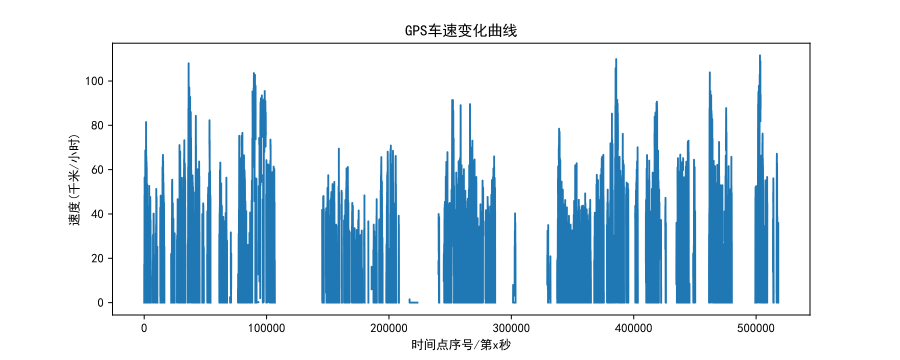
\includegraphics[width=0.9\linewidth,angle=0]{figures/data1-fill-time-speed.png}}
\subfigure[数据集2速度分布图] { 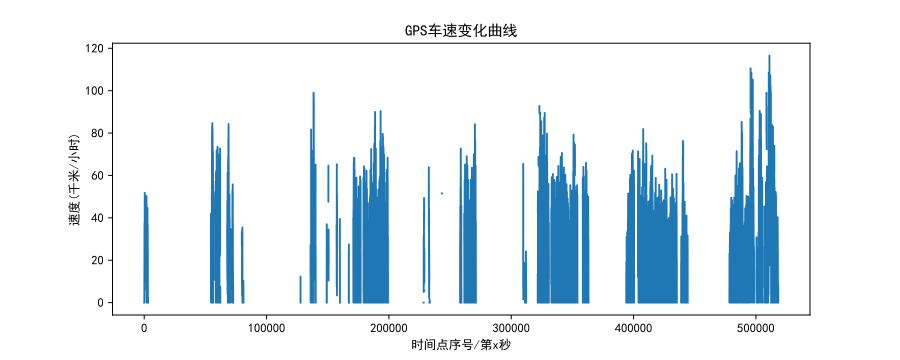
\includegraphics[width=0.9\linewidth,angle=0]{figures/data2-fill-time-speed.png}}
\subfigure[数据集3速度分布图] { 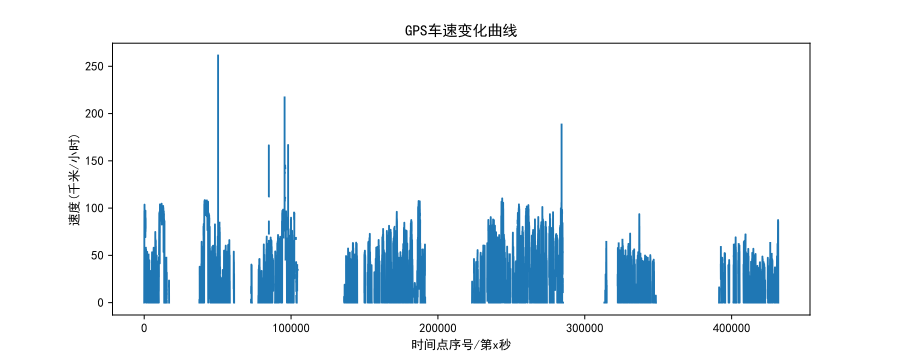
\includegraphics[width=0.9\linewidth,angle=0]{figures/data3-fill-time-speed.png}}

\caption{补全时间序列的速度分布图}
\label{f3}
\end{figure}

\strong{确定删除时间段阈值。}
观察图三中三个数据集的速度-时间分布图可以发现,图中存在许多速度空缺值,最长缺失时间长度超过5000s。因此,本文针对缺失时长大于180s的不予考虑,直接予以删除处理。对缺失时长小于180s的片段进行统计,以文件一为例,结果见下图四。
\begin{figure}[htbp] % 插入多张图片并排
\centering
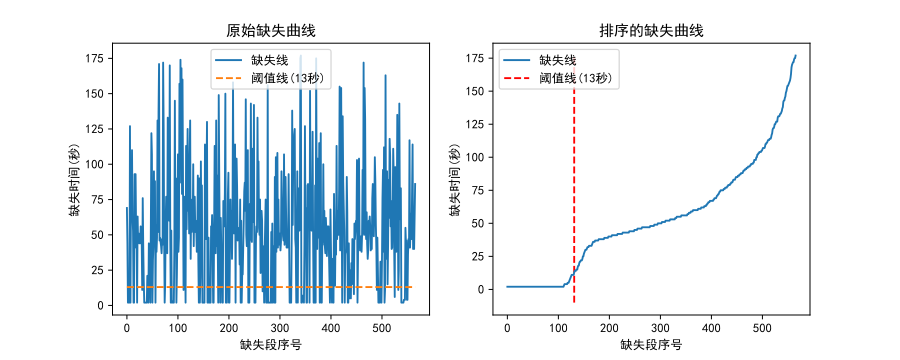
\includegraphics[width=0.9\linewidth,angle=0]{figures/data1-lack-map-curve.png}
\caption{时间缺失片段长度图}
\label{f4}
\end{figure}

观察图四分布,其中左图表示每个缺失时间段片段的分布,将其按缺失时间长度从小到大排序后得到右边的分布图。观察右图,可发现排序后的分布曲线(蓝色)存在一个快速增长区域,本文将第一次出现斜率大于1的位置取为临界点,由临界值位置确定删除时间段的阈值,从而保证保留大部分有效的数据信息。各数据文件的阈值取值结果见表2

\begin{table}[htbp]
\caption{时间段长度选择阈值}
\centering
\begin{tabular}{c c}% 通过添加 | 来表示是否需要绘制竖线
\hline  % 在表格最上方绘制横线
\makebox[0.4\textwidth][c]{文件}	& \makebox[0.4\textwidth][c]{时间段长度阈值(秒)}\\
\hline
文件1&13\\
文件2&26\\
文件3&28\\
\hline  %在第一行和第二行之间绘制横线
\end{tabular}
\end{table}

\strong{空白时间片段插值。}
删除超过阈值的时间段之后,接下来需要考虑未超过阈值的时间段,这些片段因为缺失时间长度较段,可以采用插值法进行补全。可选择的插值法包括线性插值法、三次样条插值法、拉格朗日插值法和牛顿插值法等,本文采用三次样条插值法进行插值。插值后得到的数据如图五所示。
\begin{figure}[htbp] % 插入多张图片并排
\centering
\subfigure[数据集1速度分布] { 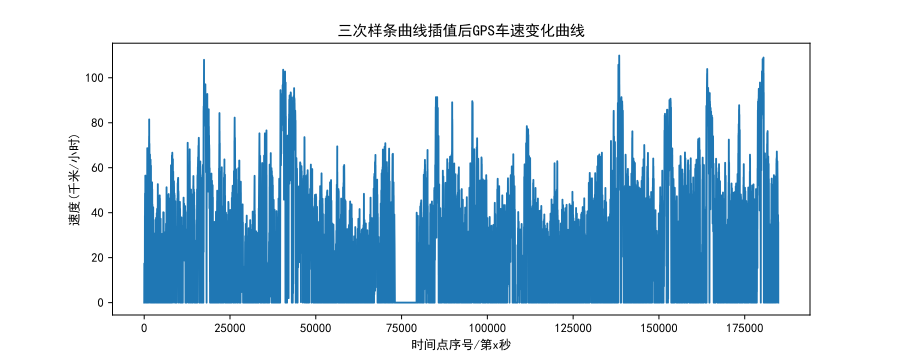
\includegraphics[width=0.9\linewidth,angle=0]{figures/data1-interpolate-spline-data-speed.png}}
\subfigure[数据集2速度分布] { 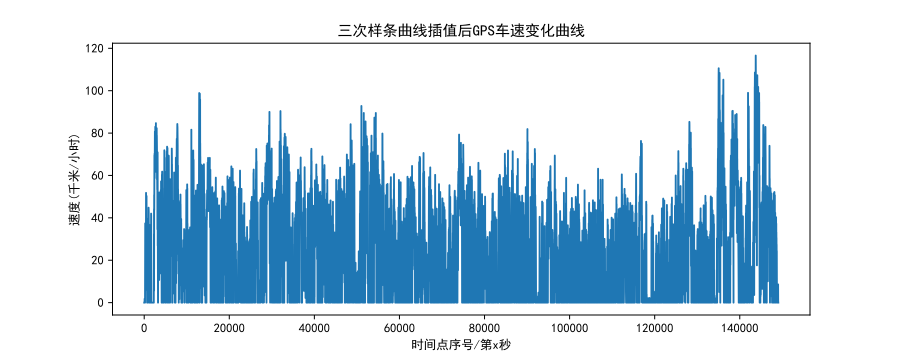
\includegraphics[width=0.9\linewidth,angle=0]{figures/data2-interpolate-spline-data-speed.png}}
\subfigure[数据集3速度分布] { 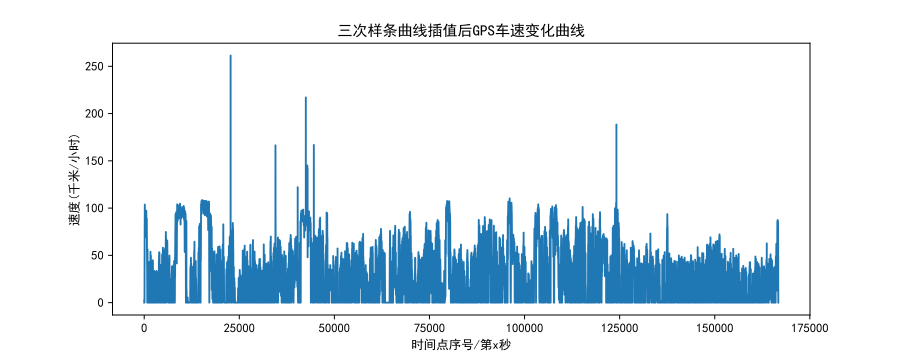
\includegraphics[width=0.9\linewidth,angle=0]{figures/data3-interpolate-spline-data-speed.png}}

\caption{插值后的速度分布图}
\label{f5}
\end{figure}

\subsubsection{加、减速度异常处理}
根据题目要求,普通轿车一般情况下的最大加速度不超过3.968 $m/s^2$,最大减速度不超过8 $m/s^2$。利用GPS车速求得各秒瞬时加速度后,筛选出不满足要求的异常点,删除后进行线性插值。如图六所示,原实测数据中蓝色线段为异常数据段,删除后在该数据缺失区间内采用线性插值使得加速度满足题目要求。同时,在发现许多数据点的GPS车速超过国家高速公路正常高速限速120km/h,最大值高达261.4km/h,不符合普通轿车行驶情况,对这部分速度异常数据进行插值替代。
\begin{figure}[htbp] % 插入多张图片并排
\centering
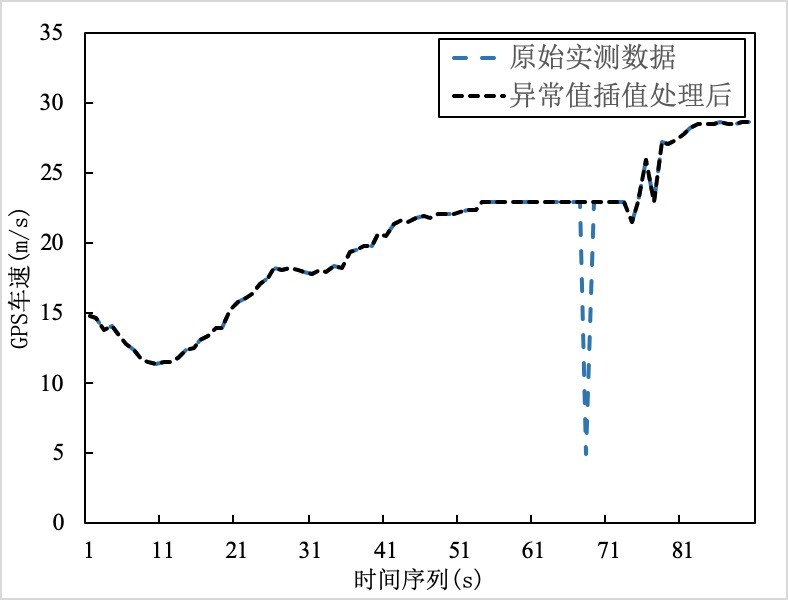
\includegraphics[width=0.9\linewidth,angle=0]{figures/acc.jpg}
\caption{加、减速度异常处理前后对比}
\label{f6}
\end{figure}

\subsubsection{长期停车、堵车问题}
\strong{长期停车问题。}
以发动机转速是否为0判断停车是否熄火,停车不熄火问题按照怠速情况处理,而停车熄火了但采集设备仍在运行情况不含有效信息,予以删除。统计发现,仅存在前者工况,不存在停车熄火问题。

\strong{堵车问题。}
题目要求,将长时间堵车、断断续续低速行驶情况(最高车速小于10km/h),按怠速情况处理,本文中,利用matlab程序遍历时间序列,寻找符合条件(车速持续小于3.968m/s且持续时长大于30s)的片段进行标记,将这类片段的车速记为0,方便后续怠速部分的处理以及运动学片段的提取。

\subsubsection{怠速时间超长问题}
怠速是指车速为零,发动机转速非零的汽车行驶状态。题目要求怠速最长时间按180秒处理,也就是压缩怠速时间超过180s时的片段区间的时间轴。统计发现,怠速时长超过180s的异常情况共出现121次,处理后的怠速时间片段共1868个,时间长度分布如图七所示。
\begin{figure}[htbp] % 插入多张图片并排
\centering
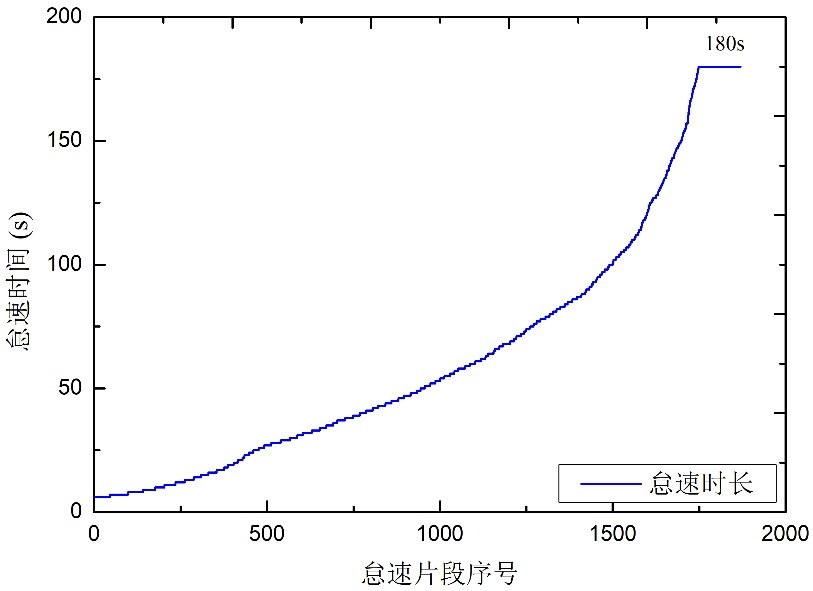
\includegraphics[width=0.9\linewidth,angle=0]{figures/dead.jpg}
\caption{怠速时间分布情况}
\label{f7}
\end{figure}

\subsubsection{数据预处理结果}
各数据文件经预处理后的记录数见表3。
\begin{table}[htbp]
\caption{各数据文件的记录数}
\centering
\begin{tabular}{c c}% 通过添加 | 来表示是否需要绘制竖线
\hline  % 在表格最上方绘制横线
\makebox[0.4\textwidth][c]{数据集1}	& \makebox[0.4\textwidth][c]{116347}\\
数据集2&108620\\
数据集3&101887\\
\hline  %在第一行和第二行之间绘制横线
\end{tabular}
\end{table}


%%%%%%%%%%%%%%%%%%%%%%%%%%%%%%%%%%%%%%%%%%%%%%%%%%%%%%%%%%%%%%%%%%%%%%%%%%
\section{问题二:运动学片段提取}
\subsection{问题分析}
针对问题二,本文基于预处理之后的车辆行驶数据先判别车辆行驶的怠速状态,进行标记后划分提取各运动学片段,片段长度小于5s予以删除,得到一个所给数据集的运动学片段的集合,得到数量总数。

编写matlab函数,遍历预处理后的数据,标记运动学片段开始、运行片段开始、运动学片段结束的时间序列,生成运动学片段指针序列。
\subsection{问题求解}
根据上述分析,使用Matlab编写程序,可得到结果如表4.

\begin{table}[htbp]
\caption{各数据文件的运动学片段数}
\centering
\begin{tabular}{c c}% 通过添加 | 来表示是否需要绘制竖线
\hline  % 在表格最上方绘制横线
\makebox[0.4\textwidth][c]{数据集1}	& \makebox[0.4\textwidth][c]{748}\\
数据集2&584\\
数据集3&537\\
\hline  %在第一行和第二行之间绘制横线
\end{tabular}
\end{table}


\section{问题三:汽车行驶工况的构建}
\subsection{问题分析}
针对问题三,本文建模步骤如下:
\begin{enumerate}
\item 根据文献\cite{c5}初步选取23个描述汽车行驶工况的特征变量,以运动学片段油耗为因变量运用相关性分析进行变量筛选,最后确定特征变量。
\item 利用主成分分析法(Principle Component Analysis,PCA)对特征参数矩阵进行降维处理,选取能够代表大部分信息的主成分。
\item 根据各运动学片段主成分的得分矩阵进行k-均值聚类,将特性相似的运动学片段划分到一个类别中。
\item 用matlab编写函数,将片段分类在总数据集中的时间占比作为各类典型运动片段的时间权值,设定所需时长1250秒,结合分类运动学片段的平均时间和总时间计算分类所需组成片段数量,分别为5和3;根据各片段与该类总特征向量的相关系数降序排列,取前5\%的运动学片段作为备选集,数量分别为58和34,两个备选集进行遍历组合,选取满足时间长度区间要求,同时总体运动学片段特征向量相关系数最大的组合作为所给数据的最优运动学片段组合。

\end{enumerate}

\subsection{问题求解}
\subsubsection{特征变量选取}
参考 TorpE 的研究,本文选取速度变量、加速度变量、驾驶路程与时间和行驶特点变量 4 大类共 23 个变量\cite{c5}。变量名与符号如表1 所示。构建行驶工况的目的之一是为了评价汽车的燃油经济性,由此本文将运动学片段的油耗量作为因变量。

\strong{相关性分析。}相关系数是评价两个变量相关程度的指标,其定义如式(1)所示:

\begin{equation}
r=\frac{\sum\limits^n_{i=1}(x_i-\bar x)(y_i-\bar y)}{\sqrt{\sum\limits^n_{i=1}(x_i-\bar x)^2\sum\limits^n_{i=1}(y_i-\bar y)^2}}
\end{equation}

其中,n为样本个数,$\bar x$ 和$\bar y$ 分别为变量x和y的平均值。

统计学上认为,相关系数的取值范围为[-1,1],当 r>0 时表示正相关,r< 0 时表示负相关,并且当相关系数$|r|\geq 0.8$ 时,可认为两变量显著线性相关。本文认为,两个变量相关系数的绝对值达到 0.8,则认为两变量高度线性相关,并保留与油耗的相关系数值较大的变量。

计算四大类变量间的相关系数矩阵,结果见表5,表6,表7和表8,f表示因变量油耗。
\begin{table}[htbp]
\caption{速度类变量相关系数表}
\centering
\begin{tabular}{c c c c c c}% 通过添加 | 来表示是否需要绘制竖线
\hline  % 在表格最上方绘制横线
r           & $v_m$	& $v_{max}$	& $v_{std}$ & $v_mr$	& f\\
\hline
$v_m$    &	1.0000&	0.8652	&0.7959	&0.8822&-0.6749\\
$v_{max}$ &	0.8652	&1.0000&	0.9472	&0.9591&	-0.3537\\
$v_{std}$ &0.7959	&0.9472&	1.0000&	0.9474&	-0.3178\\
$v_{mr}$	&0.8822	&0.9591&	0.9474&	1.0000&	-0.3340\\

\hline  %在第一行和第二行之间绘制横线
\end{tabular}
\end{table}

\begin{table}[htbp]
\caption{速度类变量相关系数表}
\centering
\begin{tabular}{c c c c c c c c c}% 通过添加 | 来表示是否需要绘制竖线
\hline  % 在表格最上方绘制横线
r & $a_{mp}$ & $a_{mn}$ & $t_{pa}$	& $t_{na}$ & $a_{std}$ & $	p_{tpa}$	& $p_{tna}$	&f\\
\hline
$a_{mp}$	 &1.0000	&0.5010	&0.3479	&0.2975	&0.8412	&0.4187	&0.2212	&0.2742\\
$a_{mn}$ &0.5010	&1.0000	&0.2073	&0.2701	&0.8171	&0.1209	&0.3353	&0.2005\\
$t_{pa} $ &0.3479	&0.2073	&1.0000	&0.9641	&0.2961	&0.5239	&0.4349	&0.3848\\
$t_{na}$ &0.2975	&0.2701	&0.9641	&1.0000	&0.3023	&0.4549	&0.4926	&0.3811\\
$a_{std}$ &0.8412	&0.8171	&-0.2961	&-0.3023	&1.0000	&-0.3013	&-0.3149	&0.2605\\
$p_{tpa}$	 &-0.4187	&0.1209	&0.5239	&0.4549	&-0.3013	&1.0000	&0.8045	&-0.6227\\
$p_{tna}$	 &-0.2212	&0.3353	&0.4349	&0.4926	&-0.3149	&0.8045	&1.0000	&-0.6197\\
\hline  %在第一行和第二行之间绘制横线
\end{tabular}
\end{table}
%%%%%%%%%%%%%%%%%%%%%%%%%%%%%%%%%%%%%%%%%%
\begin{table}[htbp]
\caption{加速度类变量相关系数表(相关系数大于0.8部分)}
\centering
\begin{tabular}{c c c c c c c c c}% 通过添加 | 来表示是否需要绘制竖线
\hline  % 在表格最上方绘制横线
r & $a_{mp}$ & $a_{mn}$ & $t_{pa}$	& $t_{na}$ & $a_{std}$ & $	p_{tpa}$	& $p_{tna}$	&f\\
\hline
$a_{mp}$	 &1.0000	&0.5010	&0.3479	&0.2975	&0.8412	&0.4187	&0.2212	&0.2742\\
$a_{mn}$ &0.5010	&1.0000	&0.2073	&0.2701	&0.8171	&0.1209	&0.3353	&0.2005\\
$t_{pa} $ &0.3479	&0.2073	&1.0000	&0.9641	&0.2961	&0.5239	&0.4349	&0.3848\\
$t_{na}$ &0.2975	&0.2701	&0.9641	&1.0000	&0.3023	&0.4549	&0.4926	&0.3811\\
$a_{std}$ &0.8412	&0.8171	&-0.2961	&-0.3023	&1.0000	&-0.3013	&-0.3149	&0.2605\\
$p_{tpa}$	 &-0.4187	&0.1209	&0.5239	&0.4549	&-0.3013	&1.0000	&0.8045	&-0.6227\\
$p_{tna}$	 &-0.2212	&0.3353	&0.4349	&0.4926	&-0.3149	&0.8045	&1.0000	&-0.6197\\
\hline  %在第一行和第二行之间绘制横线
\end{tabular}
\end{table}
%%%%%%%%%%%%%%%%%%%%%%%%%%%%%%%%%%%%%%%%%%
\begin{table}[htbp]
\caption{路程与时间类变量相关系数表}
\centering
\begin{tabular}{c c c c c}% 通过添加 | 来表示是否需要绘制竖线
\hline  % 在表格最上方绘制横线
r & s & t & $t_r$ & f\\
\hline
s	&1.0000	&0.8440	&0.9459	&-0.3266\\
t	&0.8440	&1.0000	&0.8957	&-0.1464\\
$t_r$	&0.9459	&0.8957&	1.0000	&-0.3824\\

\hline  %在第一行和第二行之间绘制横线
\end{tabular}
\end{table}
%%%%%%%%%%%%%%%%%%%%%%%%%%%%%%%%%%%%%%%%%%%%
\begin{table}[htbp]
\caption{行驶特点类变量相关系数表}
\centering
\begin{tabular}{c c c c c c c}% 通过添加 | 来表示是否需要绘制竖线
\hline  % 在表格最上方绘制横线
r	& $t_i$	& $t_c$	& $p_{ti}$ &	$p_{tc}$	&RPA	&f\\
\hline
$t_i$ &1.0000	&-0.0222&	0.5912	&-0.3860&	0.0648&	0.4483\\
$t_c$	& -0.0222&	1.0000	&-0.5083&	0.6768	&-0.2601	&-0.3430\\
$p_{ti}$ & 0.5912&	-0.5083&	1.0000&	-0.7612&	0.1781&	0.6749\\
$p_{tc}$	& -0.3860&	0.6768&	-0.7612&	1.0000	&-0.4080&	-0.5010\\
RPA	& 0.0648&	-0.2601	&0.1781&	-0.4080&	1.0000	&0.1268\\

\hline  %在第一行和第二行之间绘制横线
\end{tabular}
\end{table}

观察表5可以发现,速度类变量的两两线性相关程度都较高,其中 $v_m$ 与 $v_{max}$、$v_{mr}$的相关系数均大于0.8。同时其中平均速度与油耗的相关系数最大,所以此类变量只保留$v_m$和$v_{std}$。运用相同方法对其他三类变量进行相关分析,表6中剔除变量$a_{std}$,$t_{na}$和$p_{tna}$,表7仅保留变量$t_r$,表8中各变量相关性不强,均保留。

然后对剩下的16个变量进行相关分析,分析结果如表10。
\begin{table}[htbp]
\caption{变量跨类别两两相关系数表表(相关系数大于0.8部分)}
\centering
\begin{tabular}{c c c c c c c c c}% 通过添加 | 来表示是否需要绘制竖线
\hline  % 在表格最上方绘制横线
	& $v_m$ & $t_{pa}$	&$p_{tpa}$ &$t_r$ &$t_i$ &$t_c$ &$p_{ti}$&	f\\
\hline
$v_m$	&1.0000	&0.7381&	0.7532&0.7197&0.3141	&0.6616&	0.8021	&-0.6749\\
$t_pa$	&0.7381	&1.0000&0.5239&0.9824	&0.0195	&0.8830	&0.5863&	0.3848\\
$p_{tpa}$&	0.7532&0.5239	&1.0000	&0.4600	&0.5778&	0.3388	&0.9209	&0.6227\\
$t_r$	&0.7197&	0.9824	&0.4600&	1.0000	&0.0190	&0.9458	&0.5762&	0.3824\\
$t_i$	&0.3141&0.0195	&0.5778&0.0190	&1.0000	&0.0222	&0.5912	&0.4483\\
$t_c$	&0.6616&0.8830	&0.3388&0.9458	&-0.0222	&1.0000	&0.5083	&-0.3430\\
$p_{ti}$	&-0.8021&-0.5863&-0.9209&-0.5762&0.5912&-0.5083	&1.0000	&0.5400\\

\hline  %在第一行和第二行之间绘制横线
\end{tabular}
\end{table}
%%%%%%%%%%%%%%%%%%%%%%%%%%%%%%%%%%%%%%%%%%
根据上表,$t_r$,$t_c$和$p_{ti}$将被舍弃,至此保留了描述汽车行驶工况的13个特征变量,见表10。
\begin{table}[htbp]
\caption{变量跨类别两两相关系数表表(相关系数大于0.8部分)}
\centering
\begin{tabular}{c c c c}% 通过添加 | 来表示是否需要绘制竖线
\hline  % 在表格最上方绘制横线
$v_m$	&平均速度	&$v_{std}$	&速度标准差\\
\hline
$a_{mp}$	&平均加速度&	$a_{mn}$	&平均减速度\\
$t_{pa}$	&加速时间	&$a_{max}$	&最大加速度\\
$a_{min}$	&最大减速度	&$a_{stdp}$	&正加速度标准差\\
$a_{stdn}$	&减速度标准差&	$p_{tpa}$&加速时间比例\\
$t_i$	&怠速时间	&$p_{tc}$	&匀速时间比例\\
RPA	&相对正加速度&	&\\
\hline  %在第一行和第二行之间绘制横线
\end{tabular}
\end{table}
%%%%%%%%%%%%%%%%%%%%%%%%%%%%%%%%%%%%%%%%%%%

相关性分析发现,油耗与速度类变量均成负相关关系,这与实际情况不符,通过观察原始数据发现原因:怠速情况下的瞬时耗油大于汽车行驶状态下的油耗,这属于异常现象。但这对变量间的相关性分析影响不大,结果依旧可信。

\subsubsection{主成分分析}
主成分分析又称主分量分析,是将多个变量通过线性变换以选出较少个数重要变量的一种多元统计分析方法。即构造原变量的一系列线性组合,使各线性组合在彼此不相关的前提下,尽可能多地反映原变量的信息,即使其方差最大\cite{c3}。

表 11 的统计特征参数虽能充分反映汽车的行驶特点,但过多的特征参数增加了计算的复杂性,且表中特征参数之间具有相关性。因此,本文使用主成分分析法对变量数量进行降维、简化,构造原特征参变量的一系列互不相关的线性组合来尽可能多地反映原统计特征参数所提供的信息,从而更加合理地完成对运动学片段进行分类。

\strong{主成分分析步骤。}
\begin{enumerate}
\item 采用均值化方法对原始数据做标准化处理。为消除参数不同量纲的影响但保留各变量方差大小的信息,对原始数据采用均值化方法进行标准化处理。
\item 计算变量矩阵X的相关系数矩阵 R
\begin{equation}
R=\begin{bmatrix}
r_{11}  &  r_{12}  & \cdots\ &r_{1p}\\
r_{21}  &  r_{22}  & \cdots\ & r_{2p}\\
 \vdots   & \vdots & \ddots  & \vdots  \\
 r_{p1} & r_{p2}  & \cdots\ & r_{pp}\\
\end{bmatrix}
\end{equation}

其中,相关系数的计算如式 
\begin{equation}
r=\frac{\sum\limits^n_{i=1}(x_i-\bar x)(y_i-\bar y)}{\sqrt{\sum\limits^n_{i=1}(x_i-\bar x)^2\sum\limits^n_{i=1}(y_i-\bar y)^2}}
\end{equation}

\item 求解矩阵R的特征值$\lambda_1\geq \lambda_2\geq \cdots \geq \lambda_p > 0$ 及相应的特征向量:
\begin{equation}
\begin{matrix}
a_{1}=\begin{bmatrix}
a_{11}\\
a_{21}\\
 \vdots \\
 a_{p1}\\
\end{bmatrix}&
a_{1}=\begin{bmatrix}
a_{12}\\
a_{22}\\
 \vdots \\
 a_{p2}\\
\end{bmatrix}&\cdots&
a_{1}=\begin{bmatrix}
a_{1p}\\
a_{2p}\\
 \vdots \\
 a_{pp}\\
\end{bmatrix}

\end{matrix}
\end{equation}

\item 计算主成分F:
$F_i=a_{1i}X_1+a_{2i}X_2+\cdots +a_{pi}X_p$

\item 主成分选择

主成分的选择取决于保留成分的累计方差在总体方差中所占的比值,即主成分的累计贡献率。一般取累计贡献率达85-95\%的特征值$\lambda_1,\lambda_2,\cdots ,\lambda_m$所对应的第一、第二、…、第m($m\leq p$ )个主成分。为了保证主成分不丢失主要的信息,本章要求保留的主成分的累计贡献率达到 85\%。

各主成分贡献率:
\begin{equation}
\frac{\lambda_i}{\sum\limits^p_{k=1}\lambda_k},(i=1,2,\cdots,p)
\end{equation}
累积贡献率:
\begin{equation}
\frac{\sum\limits^i_{k=i}\lambda_k}{\sum\limits^p_{k=1}\lambda_k},(i=1,2,\cdots,p)
\end{equation}
\end{enumerate}

\strong{主成分分析结果。}

利用 MATLAB 编程计算每一个运动片段的特征参数,得到特征运动学片段数据集的参数矩阵。对经过均值化处理的特征参数矩阵进行主成分分析,得到了主成分的载荷矩阵、得分矩阵以及用于解释方差的特征值向量。载荷矩阵描述了原始变量与主成分的线性变换关系,某个参数在某个主成分上的载荷系数的绝对值越大,则说明该参数与该主成分的相关系数越大\cite{c4};得分矩阵为原始数据在主成分坐标系中的坐标;特征值向量记录了每一个主成分向量对应的特征值,特征值越大,表明解释的方差越大,对应主成分的贡献率越大。

图八为前8个成分贡献率帕累托图,图中曲线表示了主成分累计可以解释方差。其中前 5个成分的累计贡献率为85.1\%,保留前 5主成分,则原来由 13个特征参数表示的运动学片段数据转变为由5个主成分来描述,实现了特征参数降维。
\begin{figure}[htbp] % 插入多张图片并排
\centering
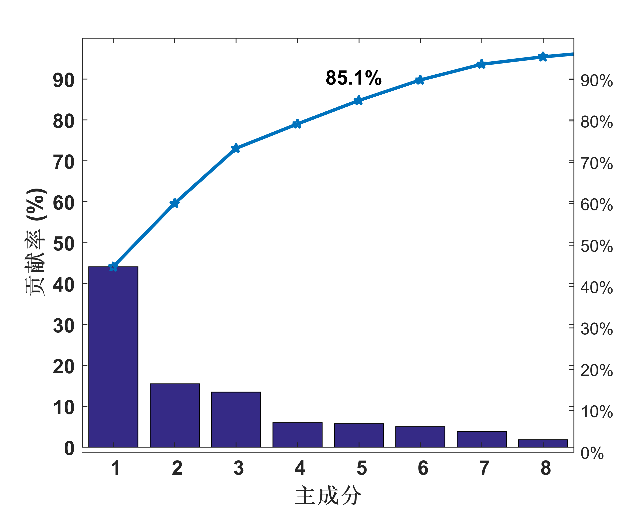
\includegraphics[width=0.9\linewidth,angle=0]{figures/pca.png}
\caption{主成分贡献率}
\label{f7}
\end{figure}

表 12为主成分的载荷矩阵,由荷载系数值可知,第一主成分主要反映平均速度$v_m$和加速时间$t_{pa}$,第二主成分主要反映怠速时间$t_i$,第三主成分主要反映平均减速度$a_{mn}$,第四主成分主要反映平均加速度$a_{mp}$和加速时间$t_{pa}$,第五主成分主要反映匀速时间比例$p_{tc}$。
\begin{table}[htbp]
\caption{主成分的载荷矩阵}
\centering
\begin{tabular}{c c c c c c}% 通过添加 | 来表示是否需要绘制竖线
\hline  % 在表格最上方绘制横线
特征变量&	F1	&F2	&F3&	F4&	F5\\
\hline
$v_m$	&0.4920	&0.0157	&-0.1377	&-0.1577&	-0.0334\\
$v_{std}$	&0.2423&	0.1532&	-0.0525&	-0.3847&	-0.0645\\
$a_{mp}$	&-0.1681&	0.1319&	-0.2492&	0.4460	&-0.1061\\
$a_{mn}$	&-0.1063&	0.2506&	-0.4181&	-0.0855&	-0.2479\\
$t_{pa}$	&0.6269&	0.3727	&0.2081	&0.4485	&-0.2647\\
$a_{max}$&	0.0214&	0.1370	&-0.1175&	0.2442&	0.1401\\
$a_{min}$&	0.0990&	0.3165	&-0.2881&	-0.088&9	0.2282\\
$a_{stdp}$&	-0.1379&	0.1307	&-0.1891&	0.4663&	0.2965\\
$a_{stdn}$&	-0.0117&	0.3174	&-0.3683&	-0.2403&	0.4004\\
$p_{tpa}	$&0.2529	&-0.1307	&-0.2029&	-0.1705&	-0.1855\\
$t_i$	&-0.1575	&0.6260&	0.5501	&-0.1951&	0.1952\\
$p_{tc}$&	0.3773	&-0.2461&	-0.0541&	0.0732&	0.6014\\
RPA	&-0.0786	&0.2254	&-0.2885	&-0.0678&	-0.3127\\
\hline  %在第一行和第二行之间绘制横线
\end{tabular}
\end{table}
%%%%%%%%%%%%%%%%%%%%%%%%%%%%%%

PCA 分析的最终结果即为 score 矩阵的前五列,该矩阵用五个主成分指标来描述每一个运动学片段的特性,减小了聚类收敛的难度,见表13。
\begin{table}[htbp]
\caption{主成分的载荷矩阵}
\centering
\begin{tabular}{c c c c c c}% 通过添加 | 来表示是否需要绘制竖线
\hline  % 在表格最上方绘制横线
&	F1	&F2	&F3&	F4&	F5\\
\hline
1&1.3240&	1.1838&	-2.0876&	0.0024&	0.2830\\
2&3.5956&	3.1691&	-0.4555&	0.2191&	0.4849\\
3&2.3019&	2.0134&	-2.1500&	-0.2677&	0.1208\\
4&2.9826&	2.3511&	-1.1814&	-0.2978&	0.7417\\
5&3.7244&	2.0199&	-2.2644&	-0.3638&	1.4108\\
$\cdots$&	$\cdots$ &$\cdots$	&$\cdots$ &	$\cdots$&$\cdots$\\
1869&2.4434	&1.4675	&-1.6804&	-0.2625&	0.6869\\

\hline  %在第一行和第二行之间绘制横线
\end{tabular}
\end{table}


\subsubsection{k-means聚类分析}
聚类分析是从数据的数值特征出发,通过分析隐含在数据中的对象及其之间的关系,来确定数据对象所属的类别。聚类分析的目的就是把相似的对象归为一类,本文将对各运动学片段的主成分得分矩阵运用 k-均值聚类的方法,对其进行分类。

它的基本思想是:首先从n个数据对象中随机选择k个对象做为初始聚类中心,然后将剩余的每个对象根据与这些聚类中心的距离,分别赋予与其距离最近的聚类。再重新计算每个所获新聚类的聚类中心(即该聚类所有对象的平均值),不断重复,直到聚类中心值不再变化(也就是准则函数开始收敛为止)。通常采用平方误差准则,其定义如公式(7) 所示:

\begin{equation}
J=\sum\limits^C_{j=1}\sum\limits^{n_j}_{k=1}||x_k-m_j||^2
\end{equation}

其中,j=1,2,…,$m_j$是C个聚类的中心,它的值为聚类q的均值,如公式所示:
\begin{equation}
m_j=\frac{1}{n_j}\sum\limits^{n_j}_{k=1}x_k
\end{equation}

\strong{k-means聚类分析步骤}

\begin{enumerate}
\item 从n个数据对象集$\{x_1,x_2,\cdots,x_n\}$中随机选取k个对象$\{Y_1,Y_2,\cdots,Y_n\}$为初始聚类中心;
\item	计算各对象到中心对象的距离,并根据最小距离重新划分; 
\item 更新聚类的平均值,即计算每个聚类中对象的平均值;
\item	循环(2)到(3),直到每个聚类不再发生变化时算法终止。

\end{enumerate}

\strong{k-均值聚类效果评价}\newline
根据K-均值聚类分析结果,运用Silhouette函数绘制轮廓图,从轮廓图上判断每个运动学片段的分类是否理\cite{c5}。其中Silhouette 函数的定义如下:
\begin{equation}
L(i)=\frac{min(b)-a}{max[a,min(b)]}
\end{equation}

式中, a为第i个运动学片段与同类运动学片段之间的 平均距离;b为一个向量,其元素是第i个运动学片段与不同类的各运动学片段间的平均距离。

轮廓值的取值范围为[-1,1],值越大说明第 i 个点的分类越合理;当 S(i)<0 时,说明第 i 个点的分类不是最优。根据聚类的结果,绘制数据集的轮廓值图,可以直观地分析聚类的合理性。

\strong{k-means聚类效果分析}

基于特征参数的第1-5主成分,运用K-均值聚类分析方法对所有的运动学片段进行分析,得到分为两类、3类和4类的聚类分析结果,见图九。
\begin{figure}[htbp] % 插入多张图片并排
\centering
\subfigure[] { 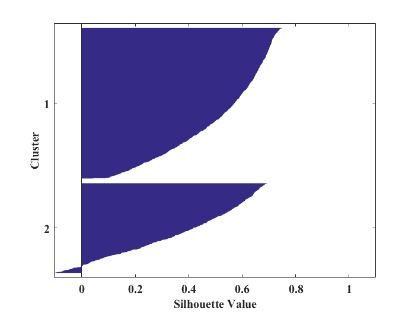
\includegraphics[width=0.3\linewidth,angle=0]{figures/c1.png}}
\subfigure[] { 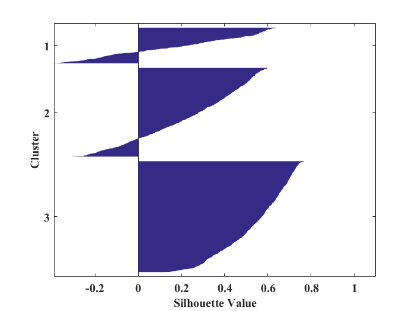
\includegraphics[width=0.3\linewidth,angle=0]{figures/c2.png}}
\subfigure[] { 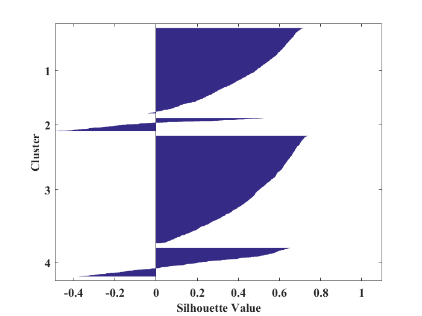
\includegraphics[width=0.3\linewidth,angle=0]{figures/c3.png}}

\caption{各聚类数轮廓图}
\label{f5}
\end{figure}

由图九可看出,当分两类时,除第2类的极少数据的Silhouette 函数值大于0外,其余数据的Silhouette 函数值均大于0,说明分类时各类型已经被很好地区分;分3类时,第1类和第2类均出现少量负值;而分4类时,第2种类和第4种类数据的Silhouette函数值均少量负值且占各类比例较大,说明聚类分析分为3类和4类时存在未被很好区分的运动学片段。根据分析结果,选取分为两类的结果作为K-均值聚类分析的最终结果,第一类包含1172个运动学片段,第二类包含698个运动学片段。

根据分析结果,选取分为两类的结果作为K-均值聚类分析的最终结果,第一类包含1172个运动学片段,第二类包含698个运动学片段。

根据聚类结果,做出各类运动片段最高速度与其概率图,如图十所示。由图可知,两类运动学片段分别代表中低速状态和高速状态,前者代表汽车在城市拥挤道路的行驶过程,后者代表汽车较为顺畅道路行驶的过程。由题目给出车辆行驶的经纬度位置可知,汽车主要在福州市和莆田市行驶,经过的路线有国道福州市仓山区G324福峡路、莆田市仙游县G324福昆线、莆田市荔城区G324城涵东大道以及福州市马尾区S1531机场高速等,也有福州市长乐区朝阳中路、福州市长乐区郑和东路等市区路线,包含了汽车在城市拥挤道路的行驶情况及汽车在较为顺畅道路的行驶情况,聚类结果与实际背景相符。
\begin{figure}[htbp] % 插入多张图片并排
\centering
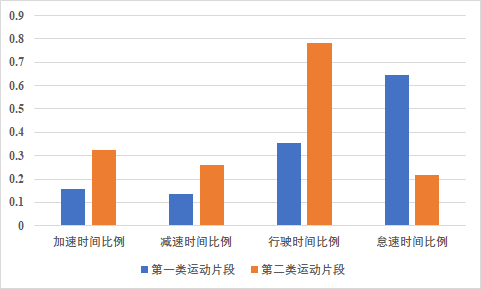
\includegraphics[width=0.9\linewidth,angle=0]{figures/rate.png}
\caption{各类运动学片段行驶状态时间比例}
\label{f5}
\end{figure}

\begin{figure}[htbp] % 插入多张图片并排
\centering
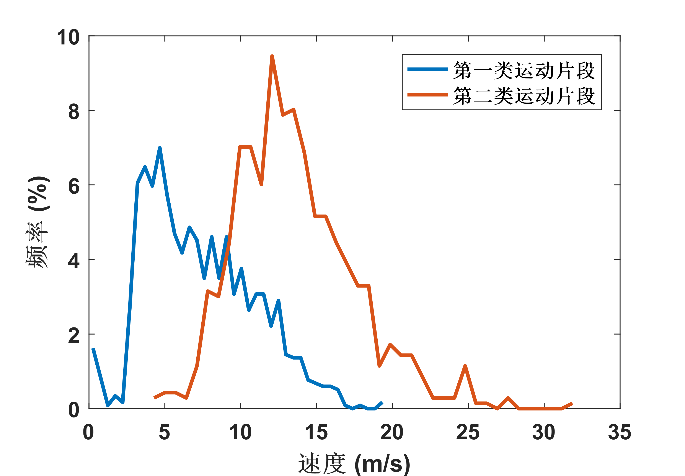
\includegraphics[width=0.9\linewidth,angle=0]{figures/max.png}
\caption{两类运动片段最高速度的概率分布图}
\label{f5}
\end{figure}

\subsubsection{典型运动片段选取}
\strong{选择步骤:}

经过以上步骤处理后,所有的运动学片段被分为2类,接下来将从2类中分别选取典型的运动学片段,筛选步骤如下:
\begin{enumerate}
\item 确定要构建工况的长度。题目要求车辆道路行驶工况的长度为 1200-1300 秒,本文先以1250s作为初始值计算。
\item 确定各类片段所需要的数量,具体计算公式:
\begin{equation}
\omega_j=\frac{1250\sum\limits^n_{k=1}t_k}{\bar T_j\sum\limits^N_{i=1}t_i}
\end{equation}
式中,$\omega_j$表示第j类片段所需要的数量,n表示第j类片段中所含有运动学片段的数量,$t_k$表示第j类片段中第k个片段的长度,$\bar T_j$表示第j类片段的平均长度,N表示在总体中所有运动学片段的个数,$t_i$表示在总体中第i个运动学片段的长度
\item 根据所分类的每类样本的综合特征参数值,分别计算此类样本中每个样本的特征参数值与该类片段总体综合特征参数值的相关系数。取相关系数前5\%的运动学片段作为典型运动学片段备选集。
\begin{equation}
\rho=\frac{Cov(X,Y)}{\sqrt{Var(X)Var(Y)}}
\end{equation}

式中Var(X)和Var(Y)分别为向量X 和向量Y 的方差,$\rho$为向量X 和向量Y 的相关系数。

\item 	在两个备选集中分别任意选取$\omega_1$和$\omega_2$个片段进行随机组合,在组合工况总时长满足1200-1300s要求的前提下选取与数据源运动学片段特征向量相关系数最大的组合作为最优的汽车行驶工况曲线。
\end{enumerate}

\strong{选取结果:}

步骤2中计算得到$\omega_1=5.1447,\omega_2=3.1191$,取整后$\omega_1=5,\omega_2=3$。

步骤3中,计算与总体综合特征参数值的相关系数时,其中 $t_{pa}$ 和 $t_i$ 表示的是加速时间总长和怠速时间总长,显然直接计算单个运动学片段和其所在类别的运动学片段集合相应值是不合理的。因此,将2类别的行程数据 $t_{pa}$和 $t_i$ 的平均值,作为其对应的总体的特征参数值。此外,为避免极端值的干扰,本章将加速度 99.5\%分位数和减速度99.5\%分位数作为特征参数代替最大加速度和最大减速度。按相关系数从大到小排序后,选取前5\%作为典型运动学片段备选集。

计算得到:第一类的典型运动学片段备选集包含58个片段,第二类的典型运动学片段备选集包含34个片段, 组合工况总时长满足1200-1300s要求的前提下,选取与数据源运动学片段特征向量相关系数最大的组合作为最优的汽车行驶工况曲线,结果见图十二。

\begin{figure}[htbp] % 插入多张图片并排
\centering
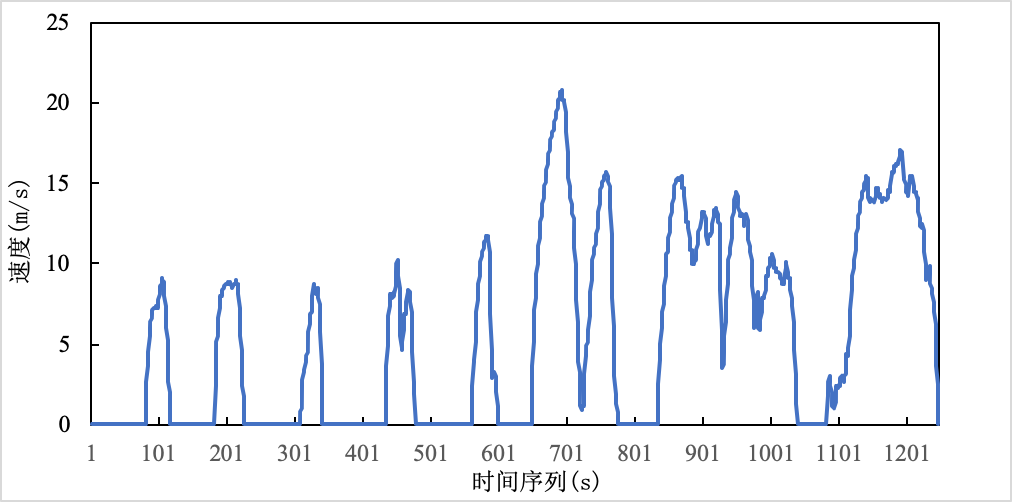
\includegraphics[width=0.9\linewidth,angle=0]{figures/final.png}
\caption{组合最优的汽车行驶工况曲线}
\label{f5}
\end{figure}
\section{汽车行驶工况评估与验证}
本章在现有条件下,通过将构建的工况与实际的工况数据进行对比分析,从特征参数和特征分布两个角度来验证行驶工况的代表性。
\subsection{特征参数误差分析}
同5.2.3的做法一样,在比较构建的工况与实际的工况数据时,用行程数据 $t_{pa}$和$ t_i$ 的平均值代替总时长,$a_{mp}$的 99.5\%分位数和$a_{mn}$的99.5\%分位数作为特征参数代替$a_{mp}$和$a_{mn}$。

由于特征参数的量纲不一致,采用平均相对误差来评价构建工况与实际工况的差异。相对误差和平均相对误差的定义如式12、13所示
\begin{equation}
diff_i=|\frac{p_{reat}-p_{cycle}}{p_{reat}}|
\end{equation}

\begin{equation}
diff_{avg}=\frac{\sum\limits^{10}_i diff_i}{10}
\end{equation}

上式中,$diff_i$表示第i个特征参数的相对误差,$p_{real}$表示实际工况的特征参数,$p_{cycle}$为构建工况的特征参数,$diff_{avg}$为平均相对误差。

根据式12计算得到构建工况各个特征参数的相对误差如表 14所示:
\begin{table}[htbp]
\caption{工况对比}
\centering
\begin{tabular}{c c c c}% 通过添加 | 来表示是否需要绘制竖线
\hline  % 在表格最上方绘制横线
&	实际工况&构建工况&相对误差\\
\hline
$v_m$	&4.8951	&4.6955	&0.0425\\
$v_{std}$	&5.4513&	4.8757	&0.1181\\
$a_{mp}$	&0.4689	&0.4887	&0.0406\\
$a_{mn}$	&-0.5770	&-0.5861	&0.0155\\
$t_{pa}$&37.2857	&37.7500	&0.0123\\
$a_{max}(99.5\%)$&	2.7778	&2.5833	&0.0753\\
$a_{min}(99.5\%)$	&-3.1666	&-3.4166	&0.0732\\
$a_{stdp}$	&0.4327&	0.4150	&0.0426\\
$a_{stdn}$	&0.5674	&0.5586&	0.0158\\
$p_{tpa}	$&0.2478	&0.2502	&0.0095\\
$t_i$	&62.8743	&64.1250	&0.0195\\
$p_{tc}$	&0.1391&	0.1234&	0.1265\\
RPA	&0.1501	&0.1617&	0.0712\\
		&&平均误差&	0.0510\\

\hline  %在第一行和第二行之间绘制横线
\end{tabular}
\end{table}

由表14可知,构建工况的特征参数都接近实际工况,最大的相对误差发生在参数$p_{tc}$上为0.1265,平均误差仅为0.05,说明构建的工况代表性很强。

\subsection{速度-加速度联合分布验证}
从工况数据速度和加速度分布的角度来评价构建工况的代表性,见图十三。由该图可知,构建工况能较好反映实际工况的速度、加速度分布特点。
\begin{figure}[htbp] % 插入多张图片并排
\centering
\subfigure[] { 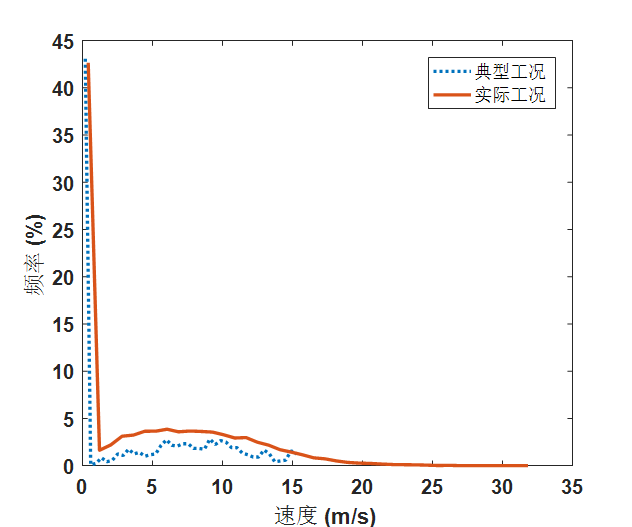
\includegraphics[width=0.45\linewidth,angle=0]{figures/61.png}}
\subfigure[] { 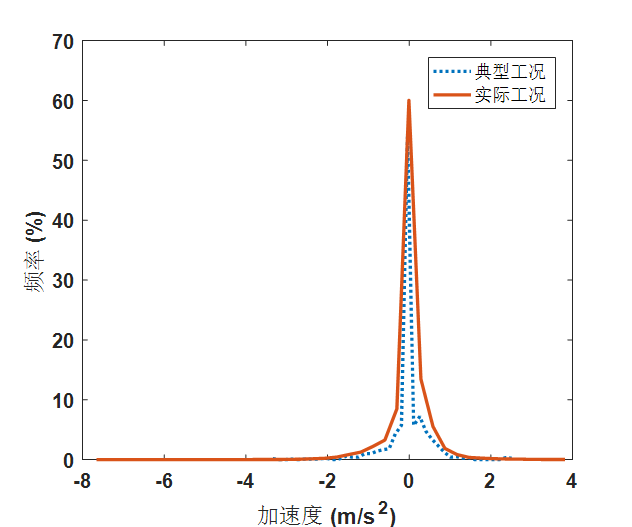
\includegraphics[width=0.45\linewidth,angle=0]{figures/62.png}}
\caption{实际工况与构建工况速度、加速度分布曲线}
\label{f5}
\end{figure}

速度分布图中,v=0 频率最大,在区间[0,2]内频率迅速减小,反映了工况平均怠速时间较长;之后随着速度增加频率逐渐增大,在[5,10]出现最大值。同时,构建工况的速度频率分布曲线在上下波动,远不如实际工况的曲线光滑,原因是实际工况的运动学片段数量远大于构建工况。而实际工况和构建工况的加速度大体上对称地分布在 a =0 两侧,且在 a =0 附近频率最大,反映出城市行驶工况具有较大的怠速比例,可能原因是长时间堵车。

为定量地评价构建工况的代表性,参考文献\cite{c6}定义了联合分布误差,见式13。 取速度的间隔值为2m/s,加速度的间隔值为 $1m/s^2$,将速度-加速度平面划分成一个个网格,则每一个小格对应于特定的速度和加速度值。统计每个小格中工况点的频率,由此得到工况的速度-加速度联合分布,见图十四。

定义速度-加速度的联合分布误差如下:
\begin{equation}
SAFD_{diff}=\frac{\sum\limits^n_i(f_{cycle,i}-f_{data,i})^2}{\sum\limits^n_if_{data.i}^2}
\end{equation}

式中,$SAFD_{diff}$表示构建工况与实际工况速度-加速度联合分布误差;i表示速度和加速度平面的第i个小格;$f_{cycle,i}$表示构建工况的第i个小格;$d_{data,i}$表示实际工况中的dii个小格;n表示网格数。

经计算,构建工况的联合分布误差为1.55\%,构建工况的代表性在特征分布方面得到验证。

\begin{figure}[htbp] % 插入多张图片并排
\centering
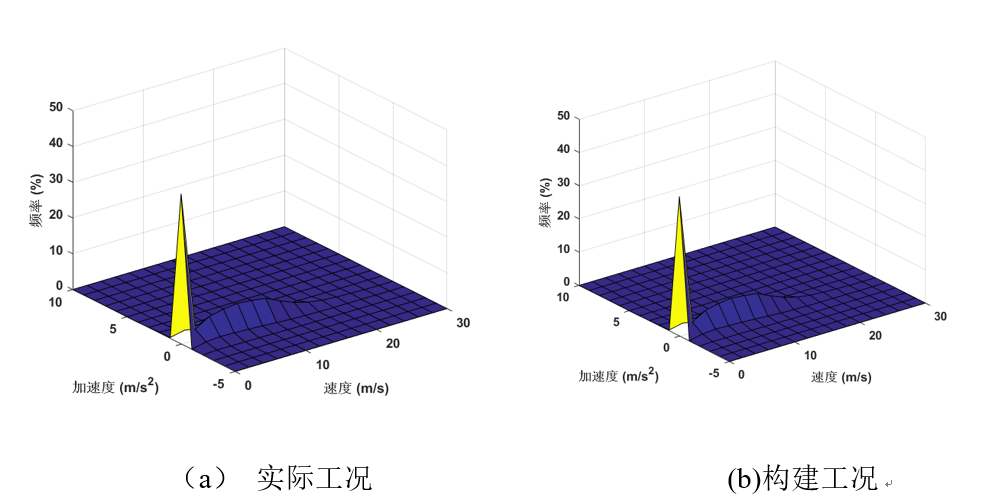
\includegraphics[width=0.7\linewidth,angle=0]{figures/qq.png}
\caption{实际工况与构建工况速度-加速度联合分布图}
\label{f5}
\end{figure}
%%%%%%%%%%%%%%%%%%%%%%%%%%%%%%%%%%%%%%%%%%%%%
%参考文献   手工录入
\newpage
\begin{thebibliography}{9}%宽度9
\bibitem[1]{c1} 张洁. 城市公共汽车行驶工况构建与研究[D]. 长安大学, 2011.
\bibitem[2]{c2} 汪雨航. 基于GPS/GIS数据的城市行驶工况构建方法研究[D]. 
\bibitem[3]{c3} 蔺宏良. 西安市交通环境轿车行驶工况与燃料消耗研究[D]. 长安大学, 2013.
\bibitem[4]{c4} 彭育辉, 杨辉宝, 李孟良, et al. 基于K-均值聚类分析的城市道路汽车行驶工况构建方法研究[J]. 汽车技术, 2017(11):17-22.
\bibitem[5]{c5} TorpE, Önnegren P. Driving cycle generation using statistical analysis and markov chains[J]. SAE Technical Paper 2013.
\bibitem[6]{c6} Brady M J, O’Mahony M. The development of a driving cycle for the greater Dublin area using a large database of driving data with a stochastic and statistical methodology[J]. ProceedingsoftheITRN2013,2013:5-
\end{thebibliography}

%采用bibtex方案
%\cite{mittelbach_latex_2004,wright_latex3_2009,beeton_unicode_2008,vieth_experiences_2009}

%\bibliographystyle{gmcm}
%\bibliography{example}


\newpage
%附录
\appendix
\setcounter{page}{1} %如果需要可以自行重置页码。
\section{源代码}
\strong{第一问补全时间序列及删选时间片段程序}
\begin{lstlisting}[language=Python]%设置不同语言即可。
import pandas as pd
import re
import datetime
import time
import matplotlib.pyplot as plt

def load_data(filename):
    '''load Excel data'''
    df = pd.read_excel(filename)
    return df
def fill_time(df):
    '''fill time'''
    df = df.set_index(['时间'])
    df = df.asfreq(freq='1S')
    return df
def _count_step(time1, time2):
    """calculate time gap"""
    return int((time2-time1).total_seconds())
def _str2time(s):
    '''transfer string to time object'''
    val = re.sub(r'\.$', '', s)
    dt = datetime.datetime.strptime(val, "%Y/%m/%d %H:%M:%S.%f")
    return dt
def transfer_data_time(df):
    '''transfer string to time object'''
    df.loc[:, '时间'] = df.loc[:, '时间'].map(_str2time)
    return df
def _find_lack_map(df):
    '''find lack time gap'''
    Lack_Map = []
    for index, row in df.iterrows():
        if index == df.index[0]:
            pre_time = index
            continue
        if _count_step(pre_time, index) > 1:
            """record start time,end time and time gap"""
            seconds = _count_step(pre_time, index)
            Lack_Map.append(
                {'start-time': pre_time, 'end-time': index, 'seconds': seconds})
        pre_time = index
    return Lack_Map
def filter_by_threshold(df, threshold):
    '''filter data by threshold'''
    lack_map = _find_lack_map(df)
    s = [lack['seconds'] for lack in lack_map]
    s2 = sorted(s)
    thres_ind = int(len(s2)*threshold)
    thres_val = s2[thres_ind]

    for lack in lack_map:
        seconds = lack['seconds']
        st_time = lack['start-time']
        end_time = lack['end-time']
        if seconds > thres_val:
            df = df.drop(df.loc[st_time:end_time].index)
    return df
def insert_data(df):
    '''insert data'''
    lack_map = _find_lack_map(df)
    s = [lack['seconds'] for lack in lack_map]
    s2 = sorted(s)
    thres_ind = int(len(s2)*threshold)
    thres_val = s2[thres_ind]
    for lack in lack_map:
        seconds = lack['seconds']
        st_time = lack['start-time']
        end_time = lack['end-time']
        if seconds < thres_val:
            time_delta = datetime.timedelta(seconds=int(seconds))
            df = df.interpolate(
                method='spline', limit_direction='forward', axis=0, order=3)
    return df
if __name__ == "__main__":
    filename = "../data/3.xlsx"
    dst_filename = "../data/3-fill-time.xlsx"
    df = load_data(filename)
    df = transfer_data_time(df)
    print('fill time...')
    df = fill_time(df)
    print('write to excel...')
    df.to_excel(dst_filename)
 \end{lstlisting}

\strong{第一问删除超过阈值点代码}
\begin{lstlisting}[language=Matlab]%设置不同语言即可。
%删除超过阈值的片段
clear;
data_del=xlsread('3-time2index-spline-3','sheet1');
gap=find(data_del(:,16)>1);%找到间隔位置
v_zero=find(data_del(:,3)==0);%找到速度为0的位置
n=length(gap);
del_row=zeros(n,2);
for i=1:n  %找到速度为0且正好最靠近间隔点的两个位置
    before=find(v_zero<=gap(i));
    del_row(i,1)=v_zero(before(end))+1;
    after=find(v_zero>gap(i));
    del_row(i,2)=v_zero(after(1))-1;
end
del_row=unique(del_row,'rows');
%根据找到的位置删除片段
data_conti(1:del_row(1,1)-1,1:16)=data_del(1:del_row(1,1)-1,1:16);
star=del_row(1,1);
for i=1:(length(del_row)-1)
    final=star+del_row(i+1,1)-del_row(i,2)-2;
    data_conti(star:final,1:16)=data_del(
(del_row(i,2)+1):(del_row(i+1,1)-1),1:16);
    star=final+1;
end
final=star+length(data_del)-del_row(end,2)-1;
data_conti(star:final,1:16)=data_del((del_row(end,2)+1):end,1:16);
data_conti(1:end,2)=1:length(data_conti);
data_conti(1:end,1)=1:length(data_conti);
cont=sum(del_row(:,2)-del_row(:,2)+1);
xlswrite('G:\数模\2019年中国研究生数学建模竞赛D题\最终数据\33-data.xlsx', data_conti);
 \end{lstlisting}

\strong{第一问筛除加速度异常程序}
\begin{lstlisting}[language=Matlab]%设置不同语言即可。
clc
clear
close all

whole_ = xlsread('1-data.xlsx');

for i = 4:length(whole_)
    if ((whole_(i-2,3)>3.968)&&(whole_(i-1,3)<-8))||...((whole_(i-2,3)<-8)
&&(whole_(i-1,3)>3.968))
        whole_(i-1,2) = (whole_(i-2,2) + whole_(i,2)) / 2;
        whole_(i-2,3) = whole_(i-1,2) - whole_(i-2,2);
        whole_(i-1,3) = whole_(i,2) - whole_(i-1,2);
    end
    if ((whole_(i-2,3)>3.968)&&(whole_(i-1,3)<0))||...((whole_(i-2,3)<0)
&&(whole_(i-1,3)>3.968))
        whole_(i-1,2) = (whole_(i-2,2) + whole_(i,2)) / 2;
        whole_(i-2,3) = whole_(i-1,2) - whole_(i-2,2);
        whole_(i-1,3) = whole_(i,2) - whole_(i-1,2);
    end
end

for i = 4:length(whole_)
    if  whole_(i-2,3) > 3.968 || whole_(i-2,3) < -8
        whole_(i-1,2) = (whole_(i-2,2) + whole_(i,2)) / 2;
        whole_(i-2,3) = whole_(i-1,2) - whole_(i-2,2);
        whole_(i-1,3) = whole_(i,2) - whole_(i-1,2);
    end
end

for i = 4:length(whole_)
    if (whole_(i-1,3)>3.968)&&(whole_(i-2,3)>3.968)
        whole_(i-1,2) = (whole_(i,2) - whole_(i-4,2)) * 3 / 4;
        whole_(i-2,2) = (whole_(i,2) - whole_(i-4,2)) * 2 / 4;
        whole_(i-3,2) = (whole_(i,2) - whole_(i-4,2)) / 4;
    end
end
for i = 2:length(whole_)
    whole_(i-1,3) =  whole_(i,2) - whole_(i-1,2);
end
xlswrite('1-data-after1_2.xlsx',whole_);

 \end{lstlisting}

\strong{第一问处理怠速情况程序}
\begin{lstlisting}[language=Matlab]%设置不同语言即可。
clc
clear
close all

whole_=xlsread('3-data-after1_2.xlsx');

a = find(whole_(:,2)<2.778);
low_v_index = [];
index_n = 0;
low_v_index(1,1)= 1;
th = 30;

for i = 2:length(a)
    if (a(i)-a(i-1)) ~= 1
        index_n = index_n + 1;
        low_v_index(index_n,2) = a(i-1);
        low_v_index(index_n + 1,1) = a(i);
        low_v_index(index_n,3) = low_v_index(index_n,2) - low_v_index(index_n,1) + 1;
    end
    if i==length(a)
        low_v_index(index_n + 1,2) = a(i);
        low_v_index(index_n + 1,3) = low_v_index(index_n + 1,2) - low_v_index(index_n  + 1,1) + 1;
    end
end   

for i = 1:length(low_v_index)
    if low_v_index(i,3) > th 
        whole_(low_v_index(i,1)+3:low_v_index(i,2)-3,2) = whole_(low_v_index(i,1)+
3:low_v_index(i,2)-3,2)*0;
    end
end


xlswrite('3-data-after1_4.xlsx',whole_);

 \end{lstlisting}

\strong{第二问提取运动学片段代码}
\begin{lstlisting}[language=Matlab]%设置不同语言即可。

clc
clear
close all

whole_=xlsread('1-data-after_2.xlsx');

index = [];
index_n = 1;
j = 1;
x=0;
while j<=length(whole_)
    %寻找第一个0点,找到跳出循环
    for i = j:length(whole_)
        if whole_(i,2) == 0
            index(index_n,1) = i;
            j = i;
            break
        end
    end
    j = j + 1;
    if j == length(whole_)
        break
    end
    %寻找后一个不为0的点
    for i = j:length(whole_)
        if whole_(i,2) ~= 0
            index(index_n,2) = i;
            j = i;
            break
        end
    end
    j = j + 1;
    if j == length(whole_)
        break
    end
   %寻找后一个为0的点
    for i = j:length(whole_)
        if whole_(i,2) == 0
            j = i;
            index(index_n,3) = i - 1;
            break
        end
    end
%怠速部分最长时间180秒
    if (index(index_n,2)-index(index_n,1))>180
        index(index_n,1) = index(index_n,2) - 180;
        x=x+1;
    end
    if index(index_n,2)-index(index_n,1)>3
        index_n = index_n + 1;
    end
end
[r,c]=size(index);
fid=fopen('index.txt','w');
for i=1:r
    for j=1:c
        if j==c
            fprintf(fid,'%d\n',index(i,j));%如果是最后一个,就换行
        else
            fprintf(fid,'%d\t',index(i,j));%如果不是最后一个,就tab
        end
    end

end
fclose(fid);


xlswrite('index.xlsx',index);
 \end{lstlisting}


\strong{第三问计算各运动片段的特征值及相关系数}
\begin{lstlisting}[language=Matlab]%设置不同语言即可。
%计算特征矩阵及相关系数矩阵
clear;
index=xlsread('data_after_task_2\index.xlsx','sheet1');%索引矩阵
data=xlsread('data_after_task_2\data_final.xlsx','sheet1');%数据矩阵,暂时认为第一列为速度,第二列为加速度,第三列为耗油量
num=length(index);
v_m=zeros(num,1);%平均速度
v_max=zeros(num,1);%最大速度
v_std=zeros(num,1);%速度标准差
v_mr=zeros(num,1);%平均行驶速度
a_mp=zeros(num,1);%平均加速度
a_mn=zeros(num,1);%平均减速度
t_pa=zeros(num,1);%加速时间
t_na=zeros(num,1);%减速时间
a_max=zeros(num,1);%最大加速度
a_min=zeros(num,1);%最大减速度
a_std=zeros(num,1);%加速度标准差
a_stdp=zeros(num,1);%正加速度标准差
a_stdn=zeros(num,1);%减速度标准差
p_tpa=zeros(num,1);%加速时间比例
p_tna=zeros(num,1);%减速时间比例
s=zeros(num,1);%运行距离
t=zeros(num,1);%总时长
t_r=zeros(num,1);%运行时长
t_i=zeros(num,1);%怠速时间
t_c=zeros(num,1);%匀速时间
p_ti=zeros(num,1);%怠速时间比例
p_tc=zeros(num,1);%匀速时间比例
RPA=zeros(num,1);%相对正加速度
f_o=zeros(num,1);%耗油量
for i=1:num
    p_ac=find(data(index(i,1):index(i,2),2)>0.1)+index(i,1)-1;%加速度大于0.1的编号
    n_ac=find(data(index(i,1):index(i,2),2)<-0.1)+index(i,1)-1;%加速度小于0.1的编号
    u_ac=find(abs(data(index(i,1):index(i,2),2))>0.1)+index(i,1)-1;%变速的编号
    z_ac=find(abs(data(index(i,3):index(i,2),2))<0.1)+index(i,3)-1;%匀速的编号
    s(i,1)=sum(data(index(i,1):index(i,2),1));
    if ~isempty(p_ac)
        a_mp(i,1)=mean(data(p_ac,2));
        t_pa(i,1)=length(p_ac);
        a_stdp(i,1)=std(data(p_ac,2));
        RPA(i,1)=sum(data(p_ac,2).*data(p_ac,1))/s(i,1);
    end
    if ~isempty(n_ac)
        a_mn(i,1)=mean(data(n_ac,2));
        t_na(i,1)=length(n_ac);
        a_stdn(i,1)=std(data(n_ac,2));
    end
    if ~isempty(u_ac)
        a_std(i,1)=std(data(u_ac,2));
    end
    if ~isempty(z_ac)
        t_c(i,1)=length(z_ac);
    end
    v_m(i,1)=mean(data(index(i,1):index(i,2),1));
    v_max(i,1)=max(data(index(i,1):index(i,2),1));
    v_std(i,1)=std(data(index(i,1):index(i,2),1));
    v_mr(i,1)=mean(data(index(i,3):index(i,2),1));
    a_max(i,1)=max(data(index(i,1):index(i,2),2));
    a_min(i,1)=min(data(index(i,1):index(i,2),2));
    p_tpa(i,1)=t_pa(i,1)/(index(i,2)-index(i,1)+1);
    p_tna(i,1)=t_na(i,1)/(index(i,2)-index(i,1)+1);
    t(i,1)=index(i,2)-index(i,1)+1;
    t_r(i,1)=index(i,2)-index(i,3)+1;
    t_i(i,1)=index(i,3)-index(i,1);
    p_ti(i,1)=t_i(i,1)/t(i,1);
    p_tc(i,1)=t_c(i,1)/t(i,1);
    f_o(i,1)=sum(data(index(i,1):index(i,2),3))/t(i,1);
end
e_value=[v_m v_max v_std v_mr a_mp a_mn t_pa t_na a_max a_min  a_std  a_stdp  a_stdn  p_tpa p_tna s t t_r t_i t_c p_ti p_tc RPA f_o];%特征值矩阵
r=zeros(length(e_value(1,:)),length(e_value(1,:)));%相关系数矩阵
for i=1:length(e_value(1,:))
    for j=i:length(e_value(1,:))
    r(i,j)=corr(e_value(:,i),e_value(:,j),'type','pearson');
    end
end
r=r+r'-eye(length(e_value(1,:)));
%xlswrite('G:\数模\2019年中国研究生数学建模竞赛D题\最终数据\1-特征矩阵.xlsx', e_value);
%xlswrite('G:\数模\2019年中国研究生数学建模竞赛D题\最终数据\1-相关系数矩阵.xlsx', r);
 \end{lstlisting}

\strong{第三问主成分分析与聚类分析}
\begin{lstlisting}[language=Matlab]%设置不同语言即可。

%主成分分析并计算轮廓值
clear;
e_value=xlsread('特征矩阵筛选.xlsx','sheet1');
size_e_value=size(e_value);
sta_e_value=zeros(size_e_value(1),size_e_value(2));
for j=1:size_e_value(2)%均值化特征矩阵
    ave_e_value_j=mean(e_value(:,j));
    for i=1:size_e_value(1)
        sta_e_value(i,j)=e_value(i,j)/ave_e_value_j;
    end
end
%sta_e_value=zscore(e_value);%标准化特征值矩阵

[coeff,score,latent,tsquare]=princomp(sta_e_value);%主成分分析
contri=(100*latent'/sum(latent'))';%各成分贡献值
score=sta_e_value*coeff(:,1:5);%主成分得分矩阵
K=2;%类的数量
Idx=kmeans(score,K);%聚类分析
list=1:K;
ave_e_value=zeros(K,length(e_value(1,:)));%各类特征平均值
SS=zeros(length(e_value),1);%各点轮廓值
for i=1:K
    kind_i=find(Idx==i);
    S=0;
    for j=1:length(kind_i)
        a_j=repmat(score(kind_i(j,:),:),[length(kind_i),1]);
        subs_i=score(kind_i,:)-a_j;
        ave_a(j,i)=sum(diag(sqrt(subs_i*subs_i')))/(length(kind_i)-1);
        other_i=find(list~=i);
        for k=1:length(other_i)
            kind_k=find(Idx==other_i(k));
            a_k=repmat(score(j,:),[length(kind_k),1]);
            subs_k=score(kind_k)-a_k;
            ave_b(j,k,i)=sum(diag(sqrt(subs_k*subs_k')))/(length(kind_k));
        end
        S(j,1)=(min(ave_b(j,:,i))-ave_a(j,i))/max([ave_a(j,i) min(ave_b(j,:,i))]);
    end
    SS(kind_i,1)=S;
    ave_e_value(i,:)=mean(e_value(kind_i,:));
end
silhouette(score,Idx);
 \end{lstlisting}

\strong{第三问计算组合片段的特征值}
\begin{lstlisting}[language=Matlab]%设置不同语言即可。
function e_value=cal_value(data_all,num)
v_m=0;%平均速度
v_std=0;%速度标准差
a_mp=0;%平均加速度
a_mn=0;%平均减速度
t_pa=0;%加速时间
a_max=0;%最大加速度
a_min=0;%最大减速度
a_stdp=0;%正加速度标准差
a_stdn=0;%减速度标准差
p_tpa=0;%加速时间比例
t_i=0;%怠速时间
p_tc=0;%匀速时间比例
RPA=0;%相对正加速度
i=1;
    p_ac=find(data_all(:,2)>0.1);%加速度大于0.1的编号
    n_ac=find(data_all(:,2)<-0.1);%加速度小于0.1的编号
    u_ac=find(abs(data_all(:,2))>0.1);%变速的编号
    z_ac=find(abs(data_all(:,2))<0.1&data_all(:,1)~=0);%匀速的编号
    s(i,1)=sum(data_all(:,1));
    if ~isempty(p_ac)
        a_mp(i,1)=mean(data_all(p_ac,2));
        t_pa(i,1)=length(p_ac);
        a_stdp(i,1)=std(data_all(p_ac,2));
        RPA(i,1)=sum(data_all(p_ac,2).*data_all(p_ac,1))/s(i,1);
    end
    if ~isempty(n_ac)
        a_mn(i,1)=mean(data_all(n_ac,2));
        t_na(i,1)=length(n_ac);
        a_stdn(i,1)=std(data_all(n_ac,2));
    end
    if ~isempty(u_ac)
        a_std(i,1)=std(data_all(u_ac,2));
    end
    if ~isempty(z_ac)
        t_c(i,1)=length(z_ac);
    end
    v_m(i,1)=mean(data_all(:,1));
    v_max(i,1)=max(data_all(:,1));
    v_std(i,1)=std(data_all(:,1));
    v_mr(i,1)=mean(data_all(:,1));
    a_max(i,1)=max(data_all(:,2));
    a_min(i,1)=min(data_all(:,2));
    t(i,1)=length(data_all);
    p_tpa(i,1)=t_pa(i,1)/t(i,1);
    p_tna(i,1)=t_na(i,1)/t(i,1);
    t_r(i,1)=length(find(data_all(:,1)~=0));
    t_i(i,1)=length(find(data_all(:,1)==0));
    p_ti(i,1)=t_i(i,1)/t(i,1);
    p_tc(i,1)=t_c(i,1)/t(i,1);
    t(i,1)=t(i,1)/num;
    t_i(i,1)=t_i(i,1)/num;
    t_pa(i,1)=t_pa(i,1)/num;
e_value=[v_m  v_std a_mp a_mn t_pa a_max a_min  a_stdp  a_stdn  p_tpa t_i p_tc RPA];%特征值矩阵
end
 \end{lstlisting}


\strong{第三问构建工况曲线代码}
\begin{lstlisting}[language=Matlab]%设置不同语言即可。

clc
clear
 
whole_= xlsread('tzjz.xlsx');
index = xlsread('jlfx.xlsx');
data_final = xlsread('data_final.xlsx');
cat_tz = xlsread('cat_TZ.xlsx');
 
 
tz1 = [];
tz2 = [];
n = 0;
l = 0;
[pd_numbers,tz_numbers] = size(whole_);
 
rank = 0.97;
 
for i = 1:length(index)
    if index(i,4) == 1
        n = n + 1;
        tz1(n,:) = [whole_(i,:),index(i,1),index(i,2)];
        tz1_(n,:) = whole_(i,:);
    end
    if index(i,4) == 2
        l = l + 1;
        tz2(l,:) = [whole_(i,:),index(i,1),index(i,2)];
        tz2_(l,:) = whole_(i,:);
    end

end

tz_1 = cat_tz(1,:);
tz_2 = cat_tz(2,:);
 
RZ_1 = [];
for i = 1:length(tz1)
    Rmat_x_y = corrcoef(tz1_(i,:),tz_1);
    RZ_1(i,:) = [tz1_(i,:),Rmat_x_y(2)]; 
end
RZ_2 = [];
for i = 1:length(tz2)
    Rmat_x_y = corrcoef(tz2_(i,:),tz_2);
    RZ_2(i,:) = [tz2_(i,:),Rmat_x_y(2)]; 
end

[y1,i1] = sort(RZ_1(:,tz_numbers + 1),'descend');
[y2,i2] = sort(RZ_2(:,tz_numbers + 1),'descend');
 
 
num_1 = floor(length(tz1) * (1 - rank));
num_2 = floor(length(tz2) * (1 - rank));
 
slected_1 = tz1(i1(1:num_1),:);
slected_2 = tz2(i2(1:num_2),:);
 
T_TOTAL = sum(tz1(:,tz_numbers + 2)-tz1(:,tz_numbers + 1)) + 
sum(tz2(:,tz_numbers + 2)-tz2(:,tz_numbers + 1));
 
 
slected_numbers_1 = 1250 * sum(tz1(:,tz_numbers + 2)-tz1(:,tz_numbers + 1)) / 
mean(tz1(:,tz_numbers + 2)-tz1(:,tz_numbers + 1)) / T_TOTAL;
slected_numbers_2 = 1250 * sum(tz2(:,tz_numbers + 2)-tz2(:,tz_numbers + 1)) / 
mean(tz2(:,tz_numbers + 2)-tz2(:,tz_numbers + 1)) / T_TOTAL;
s1 = 5;
s2 = 3;
slec_index_1 = nchoosek(1:1:num_1,s1); 

da = [slected_1(slec_index_1(1,:),:);slected_2(slec_index_2(1,:),:)];
final_d =[];
for m = 1:8
    final_d = [final_d;data_final(da(m,14):da(m,15),1:2)];
end
 
aaa=cal_value(final_d,s1+s2);
tx=0;
pd_matrix_0 = [slected_1(slec_index_1(1,:),1:tz_numbers);
slected_2(slec_index_2(1,:),1:tz_numbers)];
Rmat_pd_matrix_0 = corrcoef(aaa,cat_tz(3,:));
final_slec = [];
for i = 1:length(slec_index_1)
    for j = 2:length(slec_index_2)

            da = [slected_1(slec_index_1(i,:),:);slected_2(slec_index_2(j,:),:)];
            final_d =[];
            for m = 1:8
                final_d = [final_d;data_final(da(m,14):da(m,15),1:2)];
            end
            aaa=cal_value(final_d,s1+s2);
 
            pd_matrix = [slected_1(slec_index_1(i,:),1:tz_numbers);
slected_2(slec_index_2(j,:),
1:tz_numbers)];
            Rmat_pd_matrix =  corrcoef(aaa,cat_tz(3,:));
            
            t1 = sum(slected_1(slec_index_1(i,:),5)./slected_1(slec_index_1(i,:),10)) ;
                
            t2 = sum(slected_2(slec_index_2(j,:),5)./slected_2(slec_index_2(j,:),10)) ;
            
            
            if (Rmat_pd_matrix(2) > Rmat_pd_matrix_0(2)) && (t1 > 562) && (t1 < 608) &&...
                                                            (t2 > 638) && (t2 < 692)
                tx=1;
                pd_matrix_0 = pd_matrix;
                Rmat_pd_matrix_0(2) = Rmat_pd_matrix(2);
                final_slec=[slected_1(slec_index_1(i,:),:);slected_2(slec_index_2(j,:),:)];
            end
    end
end
 
final_v = [];
for m = 1:8
    final_v = [final_v;data_final(final_slec(m,14):final_slec(m,15),1:2)];
end
xlswrite('xulie.xlsx',final_v);

 \end{lstlisting}


\end{document} 